\documentclass{sigchi}

% Use this section to set the ACM copyright statement (e.g. for
% preprints).  Consult the conference website for the camera-ready
% copyright statement.

% Copyright
\CopyrightYear{2016}
%\setcopyright{acmcopyright}
\setcopyright{acmlicensed}
%\setcopyright{rightsretained}
%\setcopyright{usgov}
%\setcopyright{usgovmixed}
%\setcopyright{cagov}
%\setcopyright{cagovmixed}
% DOI
\doi{http://dx.doi.org/10.475/123_4}
% ISBN
\isbn{123-4567-24-567/08/06}
%Conference
\conferenceinfo{CHI'16,}{May 07--12, 2016, San Jose, CA, USA}
%Price
\acmPrice{\$15.00}

% Use this command to override the default ACM copyright statement
% (e.g. for preprints).  Consult the conference website for the
% camera-ready copyright statement.

%% HOW TO OVERRIDE THE DEFAULT COPYRIGHT STRIP --
%% Please note you need to make sure the copy for your specific
%% license is used here!
% \toappear{
% Permission to make digital or hard copies of all or part of this work
% for personal or classroom use is granted without fee provided that
% copies are not made or distributed for profit or commercial advantage
% and that copies bear this notice and the full citation on the first
% page. Copyrights for components of this work owned by others than ACM
% must be honored. Abstracting with credit is permitted. To copy
% otherwise, or republish, to post on servers or to redistribute to
% lists, requires prior specific permission and/or a fee. Request
% permissions from \href{mailto:Permissions@acm.org}{Permissions@acm.org}. \\
% \emph{CHI '16},  May 07--12, 2016, San Jose, CA, USA \\
% ACM xxx-x-xxxx-xxxx-x/xx/xx\ldots \$15.00 \\
% DOI: \url{http://dx.doi.org/xx.xxxx/xxxxxxx.xxxxxxx}
% }

% Arabic page numbers for submission.  Remove this line to eliminate
% page numbers for the camera ready copy
% \pagenumbering{arabic}

% Load basic packages
\usepackage{balance}       % to better equalize the last page
\usepackage{graphics}      % for EPS, load graphicx instead 
\usepackage[T1]{fontenc}   % for umlauts and other diaeresis
\usepackage{txfonts}
\usepackage{mathptmx}
\usepackage[pdflang={en-US},pdftex]{hyperref}
\usepackage{color}
\usepackage{booktabs}
\usepackage{textcomp}

\usepackage{grffile}
\usepackage{pdfpages}

% Some optional stuff you might like/need.
\usepackage{microtype}        % Improved Tracking and Kerning
% \usepackage[all]{hypcap}    % Fixes bug in hyperref caption linking
\usepackage{ccicons}          % Cite your images correctly!
% \usepackage[utf8]{inputenc} % for a UTF8 editor only

% If you want to use todo notes, marginpars etc. during creation of
% your draft document, you have to enable the "chi_draft" option for
% the document class. To do this, change the very first line to:
% "\documentclass[chi_draft]{sigchi}". You can then place todo notes
% by using the "\todo{...}"  command. Make sure to disable the draft
% option again before submitting your final document.
\usepackage{todonotes}

% Paper metadata (use plain text, for PDF inclusion and later
% re-using, if desired).  Use \emtpyauthor when submitting for review
% so you remain anonymous.
\def\plaintitle{A Software Survey of Meeting Scheduling Applications Group 11}
\def\plainauthor{Ryan Marks, Nick Morrison, James Taylor, Trong Tran}
\def\emptyauthor{}
\def\plainkeywords{Consumer Applications; Calendaring; Novel Interfaces, Natural Language Processing}
\def\plaingeneralterms{Design, Human Factors	}

% llt: Define a global style for URLs, rather that the default one
\makeatletter
\def\url@leostyle{%
  \@ifundefined{selectfont}{
    \def\UrlFont{\sf}
  }{
    \def\UrlFont{\small\bf\ttfamily}
  }}
\makeatother
\urlstyle{leo}

% To make various LaTeX processors do the right thing with page size.
\def\pprw{8.5in}
\def\pprh{11in}
\special{papersize=\pprw,\pprh}
\setlength{\paperwidth}{\pprw}
\setlength{\paperheight}{\pprh}
\setlength{\pdfpagewidth}{\pprw}
\setlength{\pdfpageheight}{\pprh}

% Make sure hyperref comes last of your loaded packages, to give it a
% fighting chance of not being over-written, since its job is to
% redefine many LaTeX commands.
\definecolor{linkColor}{RGB}{6,125,233}
\hypersetup{%
  pdftitle={\plaintitle},
% Use \plainauthor for final version.
%  pdfauthor={\plainauthor},
  pdfauthor={\emptyauthor},
  pdfkeywords={\plainkeywords},
  pdfdisplaydoctitle=true, % For Accessibility
  bookmarksnumbered,
  pdfstartview={FitH},
  colorlinks,
  citecolor=black,
  filecolor=black,
  linkcolor=black,
  urlcolor=linkColor,
  breaklinks=true,
  hypertexnames=false
}

% create a shortcut to typeset table headings
% \newcommand\tabhead[1]{\small\textbf{#1}}

% End of preamble. Here it comes the document.
\begin{document}

\title{\plaintitle}

\numberofauthors{4}

\author{%
  \alignauthor{Ryan Marks\\
    \affaddr{001406077}\\
    \email{marksr2@mcmaster.ca}}\\
  \alignauthor{Nick Morrison\\
    \affaddr{001426613}\\
    \email{morrin2@mcmaster.ca}}\\
  \alignauthor{James Taylor\\
    \affaddr{001155663}\\
    \email{taylojlp@mcmaster.ca}}\\
  \alignauthor{Trong Tran\\
   % \affaddr{Hamilton, Canada}\\
    \email{trantp2@mcmaster.ca}}\\
}

\maketitle

\category{H.5.m.}{Applied Computing}{Enterprise applications} 
p
\begin{abstract}
A key use of human communication using computers is to plan in person meetings.
Often this requires the coordination of many users so many tools have been developed to enable this.
This report looks at several existing solutions.
\end{abstract}

\keywords{\plainkeywords}

\section{Doodle Poll}

\subsection{Description}
A scheduling system such as Doodle strives primarily to achieve one
thing: Have a group of participants reach an agreement on a time and
place to meet.

As such, there are two primary tasks a user of the system will want
to accomplish: Creating a new event and Responding to an event
invitation. This critique will focus on those two tasks.

\subsection{Critique}
\subsubsection{Creating a new event}

From a new user's perspective, Doodle does a good job at keeping its
design language (button style, icon choice etc.) in accordance with
popular modern practice. The homepage [[https://beta.doodle.com]]
lists only a few options with the most likely next step (Create a
Doodle/Create Doodle poll) made clearly the most prevalent among
them.

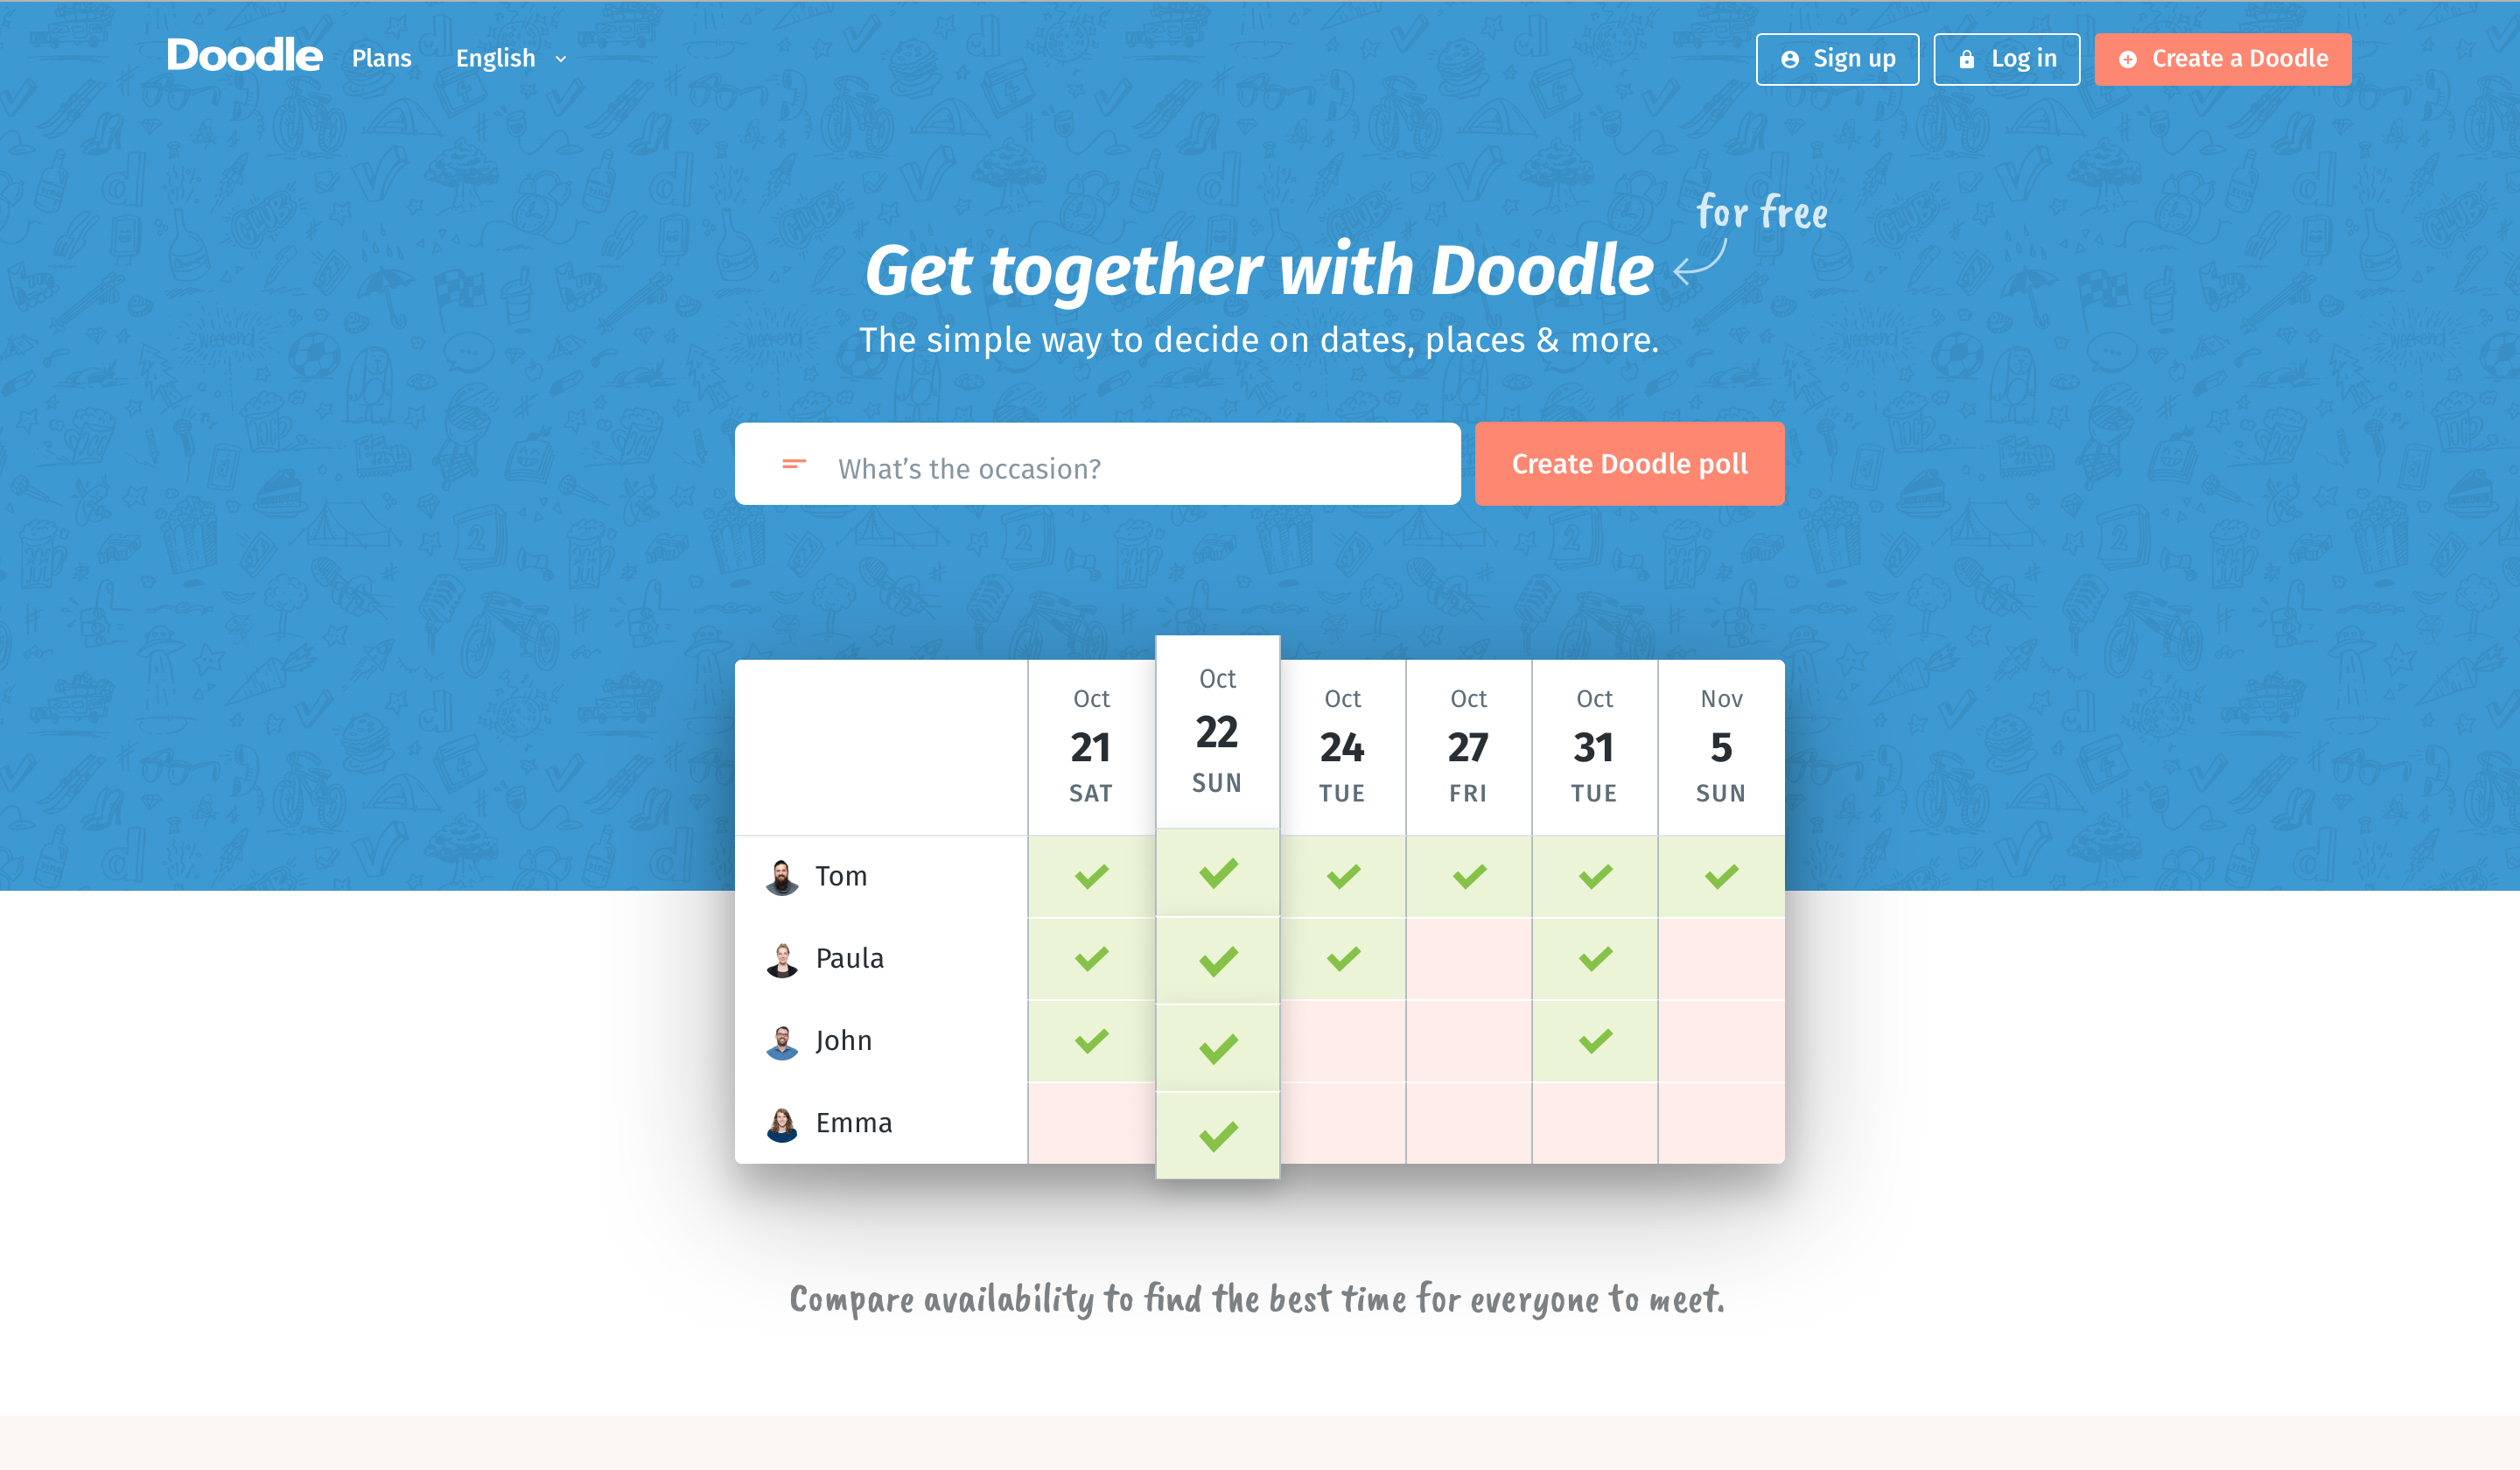
\includegraphics{doodle/index.png}

A text entry field inhabited by the "What's the occasion"
placeholder gives is given immediate focus upon loading the
page. There may be some unhelpful redundancy between the two
separate "Create Doodle poll" buttons made available. Both fulfill
nearly the exact same functionality (the difference being that the
button next to the form will populate the "Enter title" field on the
event creation page with the contents of the "What's the occasion"
text field.

[[file:create-1.png]]

The first step on the event creation page is to outline some
information about the occasion. Something lacking here is a clear
way for a user to cancel the creation of the new event. Simply
leaving the page or pressing the back button in the browser
accomplishes this, but this may not be obvious to every user.

The second step presents a dialog for selecting dates for the
event. Although the creator can select as many days as they like in
this dialog (these will be the options participants choose from),
events are effectively limited to single days. Beyond selecting
multiple adjacent (but still independent), there is no first class
method for creating an event spanning two or more days. 

[[file:create-2.png]]

After an event has been created, it is given a unique URL that can
be shared with event invitees. The creator can register to be
notified of activity within their event and is given control over
finalizing the date once she/he deems that a sufficient number of
people have voted.

** Voting on/Responding to an event invitation

Going to an event URL, an invitee is presented with the homepage for
the event. The event homepage does very little in terms of guiding
the user towards what they are meant to do. There is a somewhat
inconspicuous text field with the greyed out placeholder "Enter your
name" as well as boxes for the user to vote on the proposed
dates. Doing something as little as giving the name field focus (as
was done with the Doodle's index) would at least guide a new user in
the right direction.

[[file:event.png]]

\section{Need To Meet?}

\subsection{Critique}

\subsection{High Level Goals}

\subsection{Tasks}

\section{Google Mail/Calendar?}

\subsection{Critique}

\subsection{High Level Goals}

\subsection{Tasks}


\section{Outlook?}

\subsection{Critique}

\subsection{High Level Goals}

\subsection{Tasks}


% BALANCE COLUMNS
\balance{}

% REFERENCES FORMAT
% References must be the same font size as other body text.
\bibliographystyle{SIGCHI-Reference-Format}
\bibliography{sample}



\end{document}

%%% Local Variables:
%%% mode: latex
%%% TeX-master: t
%%% End:

